\section{Introduction}
\begin{comment}
  Very Long Baseline Interferometry (VLBI) \cite{VLBIbook} is a type of
  interferometry used in radio astronomy, in which data received at
  several telescopes is combined to produce an image with very high
  resolution. VLBI can be used for both astronomy and geodesy.  For
  astronomy, VLBI provides high-resolution images of radio sources in
  the sky, whereas in geodesy VLBI measures the location of the
  telescopes and the Earth Orientation Parameters (EOP).
\end{comment}

Recent Astronomical researches aims to study the deep-sky (farther and
farther away from us) which requires higher and higher angular
resolution to capture all the details of the observed sources.
Increasing the size of a telescope dish increases the increase the
angular resolution of the image linearly.  Nevertheless, due to
mechanical constraints, it is difficult to build moveable telescope
dishes with a size much larger than 100m. Interferometry provides a
possible solution to this problem as it permit to combine the
measurements of several telescopes to simulate a dish of size
equivalent to the maximal distance between the farthest telescopes.
This approach is called Very Large Baseline Interferometry (VLBI) and
permits us to build a virtual telescope with a dish of a size of the
earth (or more). Once the data has been recorded, the data of each
pair of stations has to be correlated.  In the \scarie\ project we are
developing and analyzing the capabilities of making a software
correlator that uses the processing power of a grid.

\scarie\ is a typical example of a recent trend of the e-Science 
community in which computation resources and scientific instruments 
are connected worldwide through high-speed networks. We think that to 
generalize the utilization of such world-size inter-connected facility, 
the grids and their middlewares have to offer services that matches the three
following user-application requirements:
\begin{itemize}
\item \emph{better performances}: an application is said performance
  limited if the resources needed to run it are not large enough to
  satisfy its needs. Performance limitations can have multiple
  origins: insufficient computing resources, memory, high network
  latency or low network throughput.
  
\item \emph{isolated environment}: there are classes of applications
  that can only be executed if put in an isolated environment in the 
  sense that the other users'application cannot interfere. Examples are 
  real-time distributed application, or benchmarks that require reproducible
  result. 

\item \emph{scheduling}: some application requires to be synchronized
  with "external events" (like having radio-telescope looking at a
  specific location in the sky at a specific date). In order to
  execute such application it is mandatory to schedule its execution 
  and reserve the needed resource in advance.
\end{itemize}
In order to fully reach the \scarie\ objectivs these three 
requirements have to be addressed for networking resource, nodes and 
data space. These are still hot-topics in the grid communauty, 
especially because networking has a long history as a 
\emph{best-effort} shared resourced which is incompatible 
with an isolated network environment. For this reason we are 
conducting ours experiences using the experimental \das3\ 
grids as it have an user-controllable dynamic photonic 
network called StarPlane to build, on demand and application specific, 
isolated virtual-network on top of the complete grid. A such service would 
permit to run \scarie\ with a good confidence level that a real-time 
experiment will not be disturbed by other users. \\

The rest of the paper is organized as follows. Section~\ref{sec:vlbi}
contains a general introduction to VLBI and its recent development 
called \evlbi. Section~\ref{sec:softwarecorrelation} describes the 
architecture of the software correlator. Section~\ref{sec:network} 
describes how the software correlator make use of the StarPlane services 
and the \das3 resources. We present benchmarks in Section~\ref{sec:benchmarks} 
and conclude the paper with future work in Section~\ref{sec:conclusion}.


\section{VLBI}\label{sec:vlbi}
In order to approximate a telescope with a larger dish, multiple
telescopes can observe the same object, and the data can be combined
using interferometry. The angular resolution of the VLBI array of
telescopes depends on the maximal projected distance between two
telescopes, while the sensitivity depends on the number of telescopes
and the bandwidth. To acquire high sensitivity data rates upto 1Gbs
per telescope are used.  The requirements on both the data streams and
the computing power to achieve a good sensitivity are shown in
Table~\ref{tab:speed}.

Traditionally, the data is recorded at the telescopes on
disk packs during a VLBI experiment. After the experiment the disks
are shipped to a central institute, e.g. the Joint Institute for VLBI
in Europe (JIVE), for correlation. At JIVE, the data from the
different telescopes is read from the disks and correlated by a
dedicated hardware correlator~\cite{EVNCorrelator}. The maximal
capacity of this hardware correlator is 16 telescopes at a data rate
of 1Gbs each.  There can be several weeks between the experiment and
the time when the correlated data becomes available.

% \marginpar{NGHK: Check 16Mb/s in table}
\begin{table}
  \centering
  \begin{tabular}[c]{|l|l|l|l|l|l|}
    \hline
    Description & \# & \#  & data-rate & spect/prod & Tflops\\
    & telescopes & sub-bands & (Mb/s) &  & \\
    \hline
    \hline
    Fabric-demo &4 &2 &16 &32 &0.16\\
    1 Gb/s, full array  &16 &16 &1024 &16 &83.39\\
    future VLBI &32 &32 &4096 &256 &\verb|~|21457\\
    \hline
  \end{tabular}
  \caption{Network bandwidths and computing power needed for an {\it e}-VLBI
    experiment based on a XF architecture.}
  \label{tab:speed}
\end{table}
\paragraph{{\it e}-VLBI}
Currently, JIVE is in the transition phase from traditional VLBI to
{\it e}-VLBI~\cite{szomoru-2004}. In an electronic VLBI ({\it e}-VLBI)
experiment, data from the telescopes is transferred directly over the
internet to JIVE, where it is streamed into the correlator in real
time. The data transport from the telescopes to JIVE goes over several
networks like local connections, paths provided by NRENs and the
G\'EANT backbone in Europe.

Transporting the data over the network has several advantages over a
traditional experiment. Obviously, the results of the experiments are
almost immediately available. This opens up the possibility to change
the course of an experiment based on earlier findings. Also, {\it
  e}-VLBI allows for real time analysis of the data and helps to
identify and resolve minor technical problems in the data collection
during the experiment.

Several experiments in the past have shown that real time {\it e}-VLBI
is possible. The EC funds the EXPReS project\footnote{EXPReS is made
  possible through the support of the European Commission (DG-INFSO),
  Sixth Framework Programme, Contract \#026642.}~\cite{EXPReS} which
aims at building a production-level {\it e}-VLBI instrument of upto 16
intercontinental telescopes connected in real-time to JIVE and
available to the general astronomy community.

\begin{figure}
  \centering
  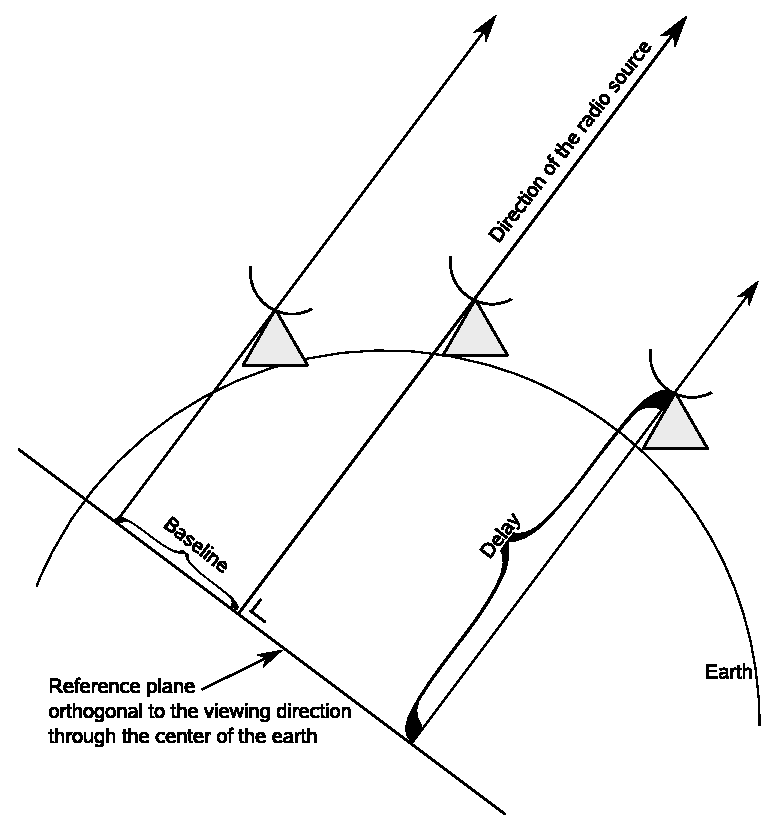
\includegraphics[width=.75\textwidth]
  {img/VLBI}
  \caption{Block diagram of the correlation.}
  \label{fig:correlation_diagram}
\end{figure}
\paragraph{Correlation}
Correlation is the process by which data from multiple telescopes is
collected and combined to measure the spatial Fourier components of
the image of the sky. The high data rates and the optimizations
complicate the process.

Assume that we are correlating the signal of two telescopes. First,
both signals are delayed to account for the different time at which
the signal arrives at the telescopes, see
Figure~\ref{fig:correlation_diagram}.  This process requires very
accurate timing information in the data and a very detailed model of
the geometry of the experiment. After the signals are properly
aligned, the signals are ready to be correlated. Correlation is a well
defined mathematical function~\cite{def_correlation} on two signals in
which the first signal is delayed with discrete steps and the integral
is computed of of the delayed signal multiplied with the second
signal. To increase the signal to noise ratio, the correlated signal
is averaged over a certain period of time. Typical averaging times lie
in the range of $0.25-4$ seconds.

For more than two stations, each station is correlated with itself
(auto-correlation) and every other station (cross-correlation). Note
that the complexity is quadratic in the number of telescopes.


%%% Local Variables:
%%% mode: latex
%%% TeX-master: "Ingrid"
%%% End:
